% Provenance (never printed): see sources/outline_sources.md (Year 2: energy geology --- the
% petroleum system quantified, unconventional resources, geothermal systems, uranium deposits,
% geological storage of carbon dioxide).
% Kerogen kinetics and elemental analyses: Fletcher and Pugmire (DOE, OSTI 1176871); kerogen
% types and Easy%Ro: Advanced Chemistry Basins Project (DOE, OSTI 830009); maturity thresholds:
% USGS MF-2008-B; TTI: Waples (1980) and Hammerschmidt et al. (2014); volumetrics and CO2
% storage: DOE/NETL (2008) and IPCC SRCCS (2005) chapter 5; geothermal: USGS OFR 2008-1296 and
% FS 2008-3082; uranium: USGS Bulletin 1693; Oklo: OSTI abstract records. Ledger rows in
% sources/ledger/book4.md; curves from figdata/bachelor-2/maturation.py and co2_density.py,
% numbers from the Book 4 second-writer scratch calculator calc/ch30.py.
% Geology and sourced numbers only: no advocacy, no policy.
\chapter{能源地质}\label{ch:b2:energy-geology}

石油是微生物遗体，与泥沙一同埋藏，经数百万年
在约 \qty{100}{\celsius} 下转化而成；地热能则是同一份地球热量，被直接取用。
二者都受温度与时间支配：前者取决于埋藏岩层缓慢升温时化学反应的进行速率，
后者取决于一定体积岩石所储存的热量，以及水将热量带到井中的快慢。
本章对含油气系统作定量分析，转而讨论缺少其中某一要素的资源，
即地热与铀矿，最后讨论其逆过程：
将二氧化碳重新封存到地下。
% ledger: earle:oil-window, earle:organic-preservation

\begin{recall}
\textbf{来自中学各册}：烃源岩、干酪根、成熟、生油窗、迁移、
储集岩、盖层、圈闭、上覆岩层、含油气系统；煤及煤阶；地热能。
\textbf{来自本科一年级分册}：热流与地温线；孔隙度与渗透率；孔隙流体
压力、有效应力和库仑判据；钻孔柱状图；沉积盆地及
沉降。\textbf{来自化学各册}：阿伦尼乌斯定律、活化能、一级
反应。\textbf{来自物理各册}：放射性衰变、衰变常数、半衰期；流体的
临界点。\textbf{来自\cref{ch:b2:basins-compared}}：\omterm{def:b2:basins-compared:curve}{沉降曲线}。
\textbf{来自\cref{ch:b2:ore-deposits}}：\omterm{def:b2:ore-deposits:types}{矿床类型}、\omterm{def:b2:ore-deposits:grade}{矿石量}。
\end{recall}

\section{含油气系统的定量分析}\label{sec:b2:energy-geology:petroleum}

含油气系统需要富含干酪根的烃源岩、储集岩、盖层、圈闭，以及足以使烃源岩受热的
上覆岩层，且各事件须按正确次序发生：石油运移时，圈闭必须已经存在。
定量分析需回答三个问题：烃源岩含何种干酪根，
干酪根已转化到何种程度，以及有多少产物
聚集在圈闭中。
% ledger: magoon00:tps

\begin{definition}[干酪根类型，范克雷维伦图]\label{def:b2:energy-geology:kerogen}
干酪根按元素组成可分为三种\emph{干酪根类型}\index{干酪根类型}：
I 型为腐泥型，氢含量最高，主要生成石油；III 型为腐殖型或煤型，
氢含量低，主要生成甲烷；II 型居中，
既可生成石油，也可生成天然气。\emph{范克雷维伦图}\index{范克雷维伦图}以干酪根的原子比 H/C
对原子比 O/C 作图；三类干酪根各占不同区域，成熟作用
使干酪根向低 H/C、低 O/C 方向移动。
\end{definition}

一项实验室研究分析了七个类型已知的未成熟干酪根，其原子比 H/C 分别为
1.51 和 1.61（I 型，其中包括犹他州的绿河油页岩，形成于湖泊，富含
藻类遗体）、1.22 至 1.28（II 型，其中包括北海的金梅里奇黏土），
1.13（II/III 混合型）和 0.99（III 型，科罗拉多州的卡梅奥煤）。绿河
干酪根，碳质量分数为 \qty{77}{\percent}，平均组成为 C$_{100}$H$_{150}$N$_3$O$_8$S：H/C 为 1.50，
O/C 为 0.08。该干酪根在实验室中以每分钟 \qty{10}{K} 加热，残余物的 H/C 降至
在 \qty{460}{\celsius} 时为 1.20，在 \qty{525}{\celsius} 时为 0.54，同时 O/C 由 0.08 降至约
0.01，其路径见下图左侧。
% ledger: acb04:kerogens, fp14:gr-kerogen, fp14:gr-chars, mf88:thresholds
% values: GR3.9 kerogen H/C 1.486, O/C 0.080; chars 460 C 1.200/0.016, 525 C 0.544/0.011 (figdata maturation.py vk)

\begin{omfigure}
\centering
\begin{minipage}[b]{0.49\linewidth}\centering
\begin{tikzpicture}
\begin{axis}[omrecord, width=0.95\linewidth, height=5.0cm, xmin=0, xmax=0.12, ymin=0, ymax=1.8,
  xlabel={原子比 O/C}, ylabel={原子比 H/C}, xtick={0,0.04,0.08}, scaled x ticks=false,
  xticklabel style={/pgf/number format/fixed}, tick label style={font=\scriptsize},
  label style={font=\small}]
% computed in figdata/bachelor-2/maturation.py part vk; ledger: fp14:gr-kerogen, fp14:gr-chars
\addplot[omThm, line width=0.9pt, mark=*, mark size=1.3pt, -{Stealth[length=4pt]}] table[x=oc, y=hc] {figdata/out/bachelor-2-maturation-vk.dat};
\node[font=\scriptsize, text=omThm, anchor=north east] at (axis cs:0.081,1.45) {干酪根};
\node[font=\scriptsize, text=omThm, anchor=west] at (axis cs:0.013,0.52) {\qty{525}{\celsius}};
% ledger: acb04:kerogens (H/C of immature kerogens; O/C not reported)
\draw[omThm, line width=1pt] (axis cs:0.104,1.51) -- (axis cs:0.12,1.51);
\draw[omThm, line width=1pt] (axis cs:0.104,1.61) -- (axis cs:0.12,1.61);
\draw[omProp, line width=1pt] (axis cs:0.104,1.22) -- (axis cs:0.12,1.22);
\draw[omProp, line width=1pt] (axis cs:0.104,1.25) -- (axis cs:0.12,1.25);
\draw[omProp, line width=1pt] (axis cs:0.104,1.28) -- (axis cs:0.12,1.28);
\draw[omExo, line width=1pt] (axis cs:0.104,1.13) -- (axis cs:0.12,1.13);
\draw[omDef, line width=1pt] (axis cs:0.104,0.99) -- (axis cs:0.12,0.99);
\node[font=\scriptsize, text=omThm, anchor=east] at (axis cs:0.103,1.58) {I};
\node[font=\scriptsize, text=omProp, anchor=east] at (axis cs:0.103,1.25) {II};
\node[font=\scriptsize, text=omDef, anchor=east] at (axis cs:0.103,0.97) {III};
\end{axis}
\end{tikzpicture}
\end{minipage}\hfill
\begin{minipage}[b]{0.49\linewidth}\centering
\begin{tikzpicture}
\begin{axis}[omrecord, width=0.95\linewidth, height=5.0cm, xmin=60, xmax=220, ymin=0, ymax=1,
  xlabel={温度（\unit{\celsius}）}, ylabel={转化率},
  tick label style={font=\scriptsize}, label style={font=\small}]
% computed in figdata/bachelor-2/maturation.py part tr; ledger: fp14:gr-daem
\addplot[black!40, densely dotted] coordinates {(60,0.5) (220,0.5)};
\addplot[omDef, line width=1.1pt] table[x=t_c, y=tr1] {figdata/out/bachelor-2-maturation-tr.dat};
\addplot[omThm, line width=1.1pt] table[x=t_c, y=tr10] {figdata/out/bachelor-2-maturation-tr.dat};
\addplot[omDef, line width=0.6pt, densely dashed] table[x=t_c, y=app1] {figdata/out/bachelor-2-maturation-tr.dat};
\addplot[omThm, line width=0.6pt, densely dashed] table[x=t_c, y=app10] {figdata/out/bachelor-2-maturation-tr.dat};
\node[font=\scriptsize, text=omDef, anchor=east] at (axis cs:125,0.80) {\qty{1}{\celsius\per\Ma}};
\node[font=\scriptsize, text=omThm, anchor=west] at (axis cs:160,0.30) {\qty{10}{\celsius\per\Ma}};
\end{axis}
\end{tikzpicture}
\end{minipage}
\par\smallskip{\small 左图为\omterm{def:b2:energy-geology:kerogen}{范克雷维伦图}，红色路径为绿河 I 型干酪根
及其在实验室中以每分钟 \qty{10}{K} 加热至 400--\qty{525}{\celsius} 后的残余物；
右侧刻度标出七个未成熟干酪根的 H/C，其类型为 I 型（红色）、II 型（橙色），
II/III 型（灰色）和 III 型（蓝色），其 O/C 未报告。数据来源：Fletcher and Pugmire（2014）；
Advanced Chemistry Basins Project（2004）。右图为绿河干酪根的转化率，
自 \qty{10}{\celsius} 起以恒定速率升温，其活化能分布
（实线），以及仅用平均能量由 \eqref{eq:b2:energy-geology:maturation} 得到的结果（虚线）。}
\end{omfigure}

干酪根向石油的转化是一组一级反应，每一个都服从
阿伦尼乌斯定律。在沉降盆地中，烃源岩的温度缓慢而几乎均匀地上升，
这使下述结果成为成熟模型的核心。

\begin{proposition}[恒定升温速率下的一级反应]\label{prop:b2:energy-geology:maturation}
设速率常数为 $k = A\,e^{-E/RT}$ 的一级反应在一种材料中进行，该材料
以恒定速率 $\beta = \mathrm{d}T/\mathrm{d}t$ 自温度 $T_0$ 起加热，此时 $k$ 可忽略。
温度为 $T$ 时未转化的分数为
\begin{equation}
x(T) = \exp\Bigl[-\frac{A}{\beta}\int_{T_0}^{T} e^{-E/RT'}\,\mathrm{d}T'\Bigr]
\approx \exp\Bigl[-\frac{A R T^2}{\beta E}\,e^{-E/RT}\Bigr] ,
\label{eq:b2:energy-geology:maturation}
\end{equation}
近似成立的条件为 $E/RT \gg 1$；转化率为 $1 - x$。
\end{proposition}

\begin{proof}
一级反应即 $\mathrm{d}x/\mathrm{d}t = -k x$。代入 $\mathrm{d}t = \mathrm{d}T/\beta$，
$\mathrm{d}\ln x = -(A/\beta)\,e^{-E/RT}\,\mathrm{d}T$，以 $x = 1$（在 $T_0$ 处）为起点积分，得第一式。
对于积分，$\frac{\mathrm{d}}{\mathrm{d}T}\bigl[\frac{RT^2}{E}e^{-E/RT}\bigr]
= \bigl(1 + \frac{2RT}{E}\bigr)e^{-E/RT}$，故积分等于 $\frac{RT^2}{E}e^{-E/RT}$，
相差一个量级为 $2RT/E$ 的相对修正，下限的贡献可忽略，因为 $e^{-E/RT_0} \ll
e^{-E/RT}$。
\end{proof}

由此得两条推论。转化发生在较窄的温度范围内，因为
$e^{-E/RT}$ 变化极快（见练习~\ref{exo:b2:energy-geology:11}）。升温较慢时转化
在较低温度下发生。取 $x = 1/2$，升温速率快十倍时，半转化温度升高
约 $(RT^2/E)\ln 10$。绿河干酪根的动力学由实验室热解数据拟合，
其 $A = \qty{9.21e13}{s^{-1}}$，$E/R = \qty{26800}{K}$（$E =
\qty{223}{kJ/mol}$）。取此单一能量，半转化温度在
\qty{1}{\celsius\per\Ma} 时为 \qty{136.4}{\celsius}，\qty{10}{\celsius\per\Ma} 时为 \qty{150.9}{\celsius}，两者相差
\qty{14.5}{\celsius}，而预测值为 $6.26 \times \ln 10 = \qty{14.4}{K}$。以
每分钟 \qty{10}{K} 加热时，同一干酪根约在 \qty{450}{\celsius} 处转化
（见练习~\ref{exo:b2:energy-geology:6}）：时间代替了温度，这正是动力学
通常在约 250 至 \qty{600}{\celsius} 下以热解测定的原因，也是把它们
外推至跨越十二个数量级的升温速率，使所预测的生油窗深度仍不确定。
% ledger: fp14:gr-daem, acb04:kinetic-spread, codata:R
% values: Thalf 136.403 / 150.873 C; RT2/E 6.2587 K; lab 445.9 C (figdata maturation.py numbers, calc/ch30.py)

实际干酪根含有强度各异的化学键，因此其动力学为活化能的分布，
各部分均服从上述命题；对绿河干酪根而言，该分布为
正态分布，标准差 $\sigma/R = \qty{481}{K}$。该分布使转化
展宽，如图右侧所示：在 \qty{150}{\celsius} 时，以 \qty{1}{\celsius\per\Ma} 升温的干酪根
已转化 \qty{93}{\percent}，升温快十倍者仅
转化 \qty{48}{\percent}。
% ledger: fp14:gr-daem
% values: TR 0.927 / 0.484 at 150 C (figdata maturation.py numbers)

\begin{definition}[镜质体反射率、时间–温度指数]\label{def:b2:energy-geology:maturity}
\emph{镜质体反射率}\index{镜质体反射率}，$R_o$，是被抛光镜质体颗粒反射的
入射光百分比；镜质体是煤和干酪根中的一种有机组分，
在显微镜下测量，它随加热不可逆地升高，记录岩石曾达到的最高热成熟度。
洛帕廷的\emph{时间–温度指数}\index{时间–温度指数}（TTI）为
$\sum_n \Delta t_n\,2^n$，对岩石所经过的各个 \qty{10}{\celsius} 区间求和，
$\Delta t_n$ 为在编号 $n$ 的区间中所经历的时间（单位为百万年），且 $n = 0$
对应 100 至 \qty{110}{\celsius}，$n = 1$ 对应 110 至 \qty{120}{\celsius}，$n = -1$ 对应 90 至
\qty{100}{\celsius}，依此类推。
\end{definition}

按反射率尺度，I 型和 II 型干酪根的生油始于 $R_o =
\qty{0.60}{\percent}$ 附近；在 1.20 至 \qty{1.30}{\percent} 以上，石油不稳定并分解为
甲烷；III 型干酪根约在 \qty{0.73}{\percent} 时开始生成甲烷，生气一直持续到
约 \qty{4.8}{\percent}。模型计算 $R_o$ 的方式与干酪根相同：Easy\%Ro 模型
将镜质体视为二十个平行的一级反应，其中 $A = \qty{e13}{s^{-1}}$，活化能
自 34 至 \qty{72}{kcal/mol}（即 142 至 \qty{301}{kJ/mol}），并将其转化分数 $F$
（至多为 0.85）映射为 $R_o = \exp(-1.6 + 3.7F)$，其范围自 0.20 至 \qty{4.7}{\percent}。
% ledger: mf88:thresholds, acb04:easyro, fp14:gr-chars

反射率沿盆地的每一层位都以相同方式计算。在下图所示的虚构盆地中，
沉积物以每百万年 \qty{100}{m} 的速率堆积，时间自 100 至 \qty{70}{\Ma}，
随后以每百万年 \qty{35}{m} 的速率堆积，地表温度为 \qty{10}{\celsius}，地温梯度恒定为
\qty{30}{\celsius\per\km}。其最老层位达到 $R_o = \qty{0.6}{\percent}$ 时，
时间为 \qty{67.6}{\Ma}，深度为 \qty{3080}{m}，温度为 \qty{102}{\celsius}；达到 \qty{1.3}{\percent} 时，
时间为 \qty{11.6}{\Ma}，深度为 \qty{5040}{m}，温度为 \qty{161}{\celsius}；现今位于 \qty{5450}{m}，
温度为 \qty{173.5}{\celsius}，$R_o = \qty{1.54}{\percent}$。由于地温线稳定，
反射率前缘几乎沿等温线延伸，生油起始温度
约为 \qty{100}{\celsius}，处于各学段分册所用的 60 至 \qty{120}{\celsius} 范围之内。
% ledger: acb04:easyro, mf88:thresholds, earle:settings, earle:oil-window
% values: figdata maturation.py numbers (oldest_ro06_*, oldest_ro13_*, ro_oldest_now)

\begin{omfigure}
\centering
\begin{tikzpicture}
\begin{axis}[omrecord, width=0.86\linewidth, height=4.8cm, xmin=0, xmax=100, ymin=0, ymax=5.6,
  x dir=reverse, y dir=reverse, ylabel={深度 (km)}, xticklabels={}, name=bh,
  tick label style={font=\scriptsize}, label style={font=\small}]
% computed in figdata/bachelor-2/maturation.py parts burial and fronts (invented basin)
\addplot[black!40, densely dashed] coordinates {(100,1.333) (0,1.333)};
\addplot[black!40, densely dashed] coordinates {(100,3.0) (0,3.0)};
\addplot[black!40, densely dashed] coordinates {(100,4.667) (0,4.667)};
\node[font=\tiny, text=black!60, anchor=south east, fill=white, inner sep=1pt] at (axis cs:1,1.333) {\qty{50}{\celsius}};
\node[font=\tiny, text=black!60, anchor=south east, fill=white, inner sep=1pt] at (axis cs:1,3.0) {\qty{100}{\celsius}};
\node[font=\tiny, text=black!60, anchor=south east, fill=white, inner sep=1pt] at (axis cs:1,4.667) {\qty{150}{\celsius}};
\addplot[black!70, line width=0.5pt, unbounded coords=jump] table[x=t_ma, y expr=\thisrow{d90}/1000] {figdata/out/bachelor-2-maturation-burial.dat};
\addplot[black!70, line width=0.5pt, unbounded coords=jump] table[x=t_ma, y expr=\thisrow{d80}/1000] {figdata/out/bachelor-2-maturation-burial.dat};
\addplot[black!70, line width=0.5pt, unbounded coords=jump] table[x=t_ma, y expr=\thisrow{d70}/1000] {figdata/out/bachelor-2-maturation-burial.dat};
\addplot[black!70, line width=0.5pt, unbounded coords=jump] table[x=t_ma, y expr=\thisrow{d60}/1000] {figdata/out/bachelor-2-maturation-burial.dat};
\addplot[black!70, line width=0.5pt, unbounded coords=jump] table[x=t_ma, y expr=\thisrow{d50}/1000] {figdata/out/bachelor-2-maturation-burial.dat};
\addplot[black!70, line width=0.5pt, unbounded coords=jump] table[x=t_ma, y expr=\thisrow{d40}/1000] {figdata/out/bachelor-2-maturation-burial.dat};
\addplot[black!70, line width=0.5pt, unbounded coords=jump] table[x=t_ma, y expr=\thisrow{d30}/1000] {figdata/out/bachelor-2-maturation-burial.dat};
\addplot[black!70, line width=0.5pt, unbounded coords=jump] table[x=t_ma, y expr=\thisrow{d20}/1000] {figdata/out/bachelor-2-maturation-burial.dat};
\addplot[black!70, line width=0.5pt, unbounded coords=jump] table[x=t_ma, y expr=\thisrow{d10}/1000] {figdata/out/bachelor-2-maturation-burial.dat};
\addplot[black, line width=1.1pt, unbounded coords=jump] table[x=t_ma, y expr=\thisrow{d100}/1000] {figdata/out/bachelor-2-maturation-burial.dat};
\addplot[omDef, line width=1.4pt, unbounded coords=jump] table[x=t_ma, y expr=\thisrow{z06}/1000] {figdata/out/bachelor-2-maturation-fronts.dat};
\addplot[omThm, line width=1.4pt, unbounded coords=jump] table[x=t_ma, y expr=\thisrow{z13}/1000] {figdata/out/bachelor-2-maturation-fronts.dat};
\node[font=\scriptsize, text=omDef, anchor=north, fill=white, inner sep=1pt] at (axis cs:40,3.05) {$R_o = \qty{0.6}{\percent}$};
\node[font=\scriptsize, text=omThm, anchor=north west, fill=white, inner sep=1pt] at (axis cs:9,5.10) {\qty{1.3}{\percent}};
\node[font=\scriptsize, anchor=north east, fill=white, inner sep=1pt] at (axis cs:58,4.75) {烃源岩};
\end{axis}
\begin{axis}[at={(bh.south west)}, anchor=north west, yshift=-0.15cm, width=0.86\linewidth,
  height=2.9cm, xmin=0, xmax=100, ymin=0.4, ymax=6.6, x dir=reverse, y dir=reverse,
  xlabel={时间 (\unit{\Ma})}, ytick={1,2,3,4,5,6},
  yticklabels={烃源岩, 储集岩, 盖层, 上覆岩层, 圈闭组, 生油},
  tick label style={font=\tiny}, label style={font=\small}, axis line style={black!60},
  xtick={100,80,60,40,20,0}]
% schematic events chart of the same invented basin
\fill[omLithShale!80!black] (axis cs:100,0.75) rectangle (axis cs:96,1.25);
\fill[omLithSand!70!black] (axis cs:90,1.75) rectangle (axis cs:85,2.25);
\fill[omLithShale!80!black] (axis cs:85,2.75) rectangle (axis cs:80,3.25);
\fill[black!25] (axis cs:80,3.75) rectangle (axis cs:0,4.25);
\fill[omProp!70] (axis cs:75,4.75) rectangle (axis cs:70,5.25);
\fill[omDef!70] (axis cs:67.6,5.75) rectangle (axis cs:11.6,6.25);
\end{axis}
\end{tikzpicture}
\par\smallskip{\small 上图：虚构盆地的埋藏史（黑色：每隔
1000 万年沉积的层位，粗线为烃源岩）、等温线（虚线），以及
Easy\%Ro 达到 \qty{0.6}{\percent}（蓝色）和 \qty{1.3}{\percent}（红色）的深度。下图为其事件图：
烃源岩中生油从 $R_o = \qty{0.6}{\percent}$ 延续至 \qty{1.3}{\percent}，
发生于圈闭形成之后。}
\end{omfigure}

TTI 方法较早，也较粗略。它假设成熟速率每升高
\qty{10}{\celsius} 便翻一番，这与活化能 $E \approx \qty{82}{kJ/mol}$ 的阿伦尼乌斯定律在
\qty{100}{\celsius} 附近的结果相符（见练习~\ref{exo:b2:energy-geology:5}）。按其标度，韦普尔斯将生油起点定在
TTI 为 15 处，高峰在 75，结束在 160。
% ledger: waples80:tti, hamm14:tti-table

\begin{method}[计算时间–温度指数]\label{met:b2:energy-geology:tti}
数据为烃源岩的埋藏史与地温线，假定地温稳定。
\begin{enumerate}
  \item \textbf{温度路径。}将各时刻的深度换算为温度：地表温度
        加上地温梯度与深度的乘积。
  \item \textbf{各区间的时间。}求每个
        \qty{10}{\celsius} 区间内所经历的时间 $\Delta t_n$；若升温速率 $\beta$ 恒定，则 $\Delta t_n = \qty{10}{\celsius}/\beta$。
  \item \textbf{求和。}按时间顺序累加乘积 $\Delta t_n\,2^n$，生油的起点、高峰和
        结束，即累加和分别越过 15、75 与 160 之时。
\end{enumerate}
\end{method}

盆地模型以转化率表示转化程度，即烃源岩原始烃类潜力中
已转化的比例。在一个加利福尼亚盆地的模型中，
假定烃源岩的排烃始于转化率 \qty{10}{\percent}，高峰位于
\qty{50}{\percent}，结束于 \qty{95}{\percent}。排出的油比水轻，
向上运移进入透水的储集岩，并在盖层封闭圈闭处聚集保存。
% ledger: peters08b4:tr, magoon00:tps, earle:migration-traps

\begin{proposition}[原地油量]\label{prop:b2:energy-geology:volumetrics}
设圈闭面积为 $A$，储层净厚度为 $h$，孔隙度为 $\phi$，含水饱和度为
$S_w$，又设 $B_o$ 为原油的体积系数，即一定量原油在储层中的体积与其
地面体积之比。
\emph{原始地质储量（地面条件）}\index{原始地质储量（地面条件）}，即地面量得的原油体积，为
\begin{equation}
\mathrm{STOIIP} = \frac{A\,h\,\phi\,(1 - S_w)}{B_o} .
\label{eq:b2:energy-geology:stoiip}
\end{equation}
\end{proposition}

\begin{proof}
储层的总体积为 $Ah$，孔隙体积为 $Ah\phi$；孔隙中比例为 $1 - S_w$ 的
部分含油，故原油在储层中占 $Ah\phi(1 - S_w)$，在地面则为此值的
$1/B_o$ 倍。
\end{proof}

\begin{definition}[采收率]\label{def:b2:energy-geology:volumetrics}
储层的\emph{采收率}\index{采收率}是指生产期内采出的油（或气）
占其原始地质储量的比例。
\end{definition}

一次采油与注水二次采油合计通常可采出地质储量中原油的 30 至 \qty{40}{\percent}；注入二氧化碳
还可再增采 10 至 \qty{15}{\percent}。一个面积为 \qty{10}{km^2}、净储层厚 \qty{30}{m} 的圈闭，
孔隙度为 0.20，含油饱和度为 0.70，$B_o = 1.2$，其所含地面原油为 \qty{3.5e7}{m^3}，
其中 1.05 至 \qty{1.4e7}{m^3} 可被采出。
% ledger: netl08:oilgas

\section{非常规资源}\label{sec:b2:energy-geology:unconventional}

\begin{definition}[非常规储层]\label{def:b2:energy-geology:unconventional}
\emph{非常规储层}\index{非常规储层}是指渗透率极低、以至其微观孔隙中的油气
若不经人工增产，便无法以经济速率流入井中的岩石；
此类储层须经沿其水平钻进的井开采，并进行
水力压裂。页岩油和页岩气保存于烃源岩本身，致密气则保存于
低渗透的砂岩与碳酸盐岩中。
\end{definition}

因此，非常规油气远景是指烃源岩或其旁侧的岩石，它们保留了其
所生成油气的一部分。所保存的产物取决于成熟度：处于生油窗内的页岩保存油，
$R_o \approx \qty{1.3}{\percent}$ 以上者保存天然气。页岩气的大规模生产始于
2000 年前后、得克萨斯州的巴内特页岩中，美国天然气产量自 2005 年以来的增长，
大部分来自页岩、砂岩、碳酸盐岩及其他致密地层中的水平钻井与水力压裂；
煤层中也可采出天然气。
% ledger: eia:shale-gas, eia:gas-coalbed, mf88:thresholds

\section{地热能}\label{sec:b2:energy-geology:geothermal}

\begin{definition}[地热系统、地热储量、焓资源类别与 EGS]\label{def:b2:energy-geology:geothermal}
\emph{地热系统}\index{地热系统}是指地壳中热量、渗透性与水同时具备的
区域，从而可由井中采出热水或蒸汽。储层的
\emph{地热储量}\index{地热储量}是指储层从其温度
冷却到参考温度时所放出的热量。\emph{高焓资源}\index{高焓资源}是指温度高于约
\qty{150}{\celsius} 的地热系统；\emph{低焓资源}\index{低焓资源}是指温度低于约
\qty{90}{\celsius} 的地热系统；介于两者之间的称为中等资源。三类资源均
适于直接利用热量，但一般只有中等和高焓两类能
用于发电。\emph{增强型地热系统}\index{增强型地热系统}（EGS）是指一块
天然渗透率低的热岩体，通过工程手段人为造出渗透性，
使水能在其中循环，并回收其热量。
\end{definition}
% ledger: usgs08g:classes, usgs08g:egs

\begin{proposition}[地热储量与可采功率]\label{prop:b2:energy-geology:heat}
设储层体积为 $V$，平均温度为 $T_R$，体积热容为 $C$（岩石与孔隙
流体合计），则其在参考温度 $T_0$ 以上所含的热量为
\begin{equation}
q_R = C\,V\,(T_R - T_0) .
\label{eq:b2:energy-geology:heat}
\end{equation}
若其中比例为 $R_g$ 的热量在生产时间 $\tau$ 内到达井口，则平均产热
功率为 $P = R_g\,q_R/\tau$。
\end{proposition}

\begin{proof}
体积元 $\mathrm{d}V$ 的温度为 $T$，放出热量 $C\,\mathrm{d}V\,(T - T_0)$，即冷却至 $T_0$；
对储层求和（设 $C$ 均匀）得 $C\,V\,(T_R - T_0)$，其中 $T_R$ 为
平均温度。功率即回收热量除以时间。
\end{proof}

资源评价采用此体积法，参考温度取 \qty{15}{\celsius}。\omterm{def:b2:energy-geology:volumetrics}{采收率}
$R_g$ 是其中的不确定部分：早期评价取 0.25，范围 0 至 0.5；来自裂缝性储层的
生产数据指向约 0.1，范围 0.05 至 0.2。取 $C = \qty{2.5}{MJ.m^{-3}.K^{-1}}$
（岩石基质为 2 至 \qty{3}{MJ.m^{-3}.K^{-1}}），一个 $3 \times 4 \times
\qty{1}{km}$、温度为 \qty{220}{\celsius} 的储层含热量 \qty{6.15e18}{J}；若 $R_g = 0.1$，开采 30 年，则
平均热功率为 \qty{650}{MW}。常规油田的发电量为每平方千米 10 至
\qty{20}{MW}。
% ledger: usgs08g:volume, delaney86b4:properties, usgs08g:egs
% values: 6.15e18 J; 6.15e17 J; 649.6 MW (calc/ch30.py)

天然\omterm{def:b2:energy-geology:geothermal}{地热系统}既需要热量，也同样需要渗透性。其中大多数主要系统位于
构造板块的边缘，与火山、喷气孔、温泉和间歇泉相伴，其渗透性通常来自
活动断层开启的裂缝：深部加热的地下水
沿这些裂缝上升，水井即从裂缝性储层中取水，如下文所述。\omterm{def:b2:energy-geology:geothermal}{增强型地热系统}无需天然储层：
其水井钻至约 \qty{5}{km}，抵达渗透性经人工改造的热岩，并
美国 2008 年的一项评估给出其初步潜力为 \qty{517800}{MW} 的
电力，而已查明的常规系统为 \qty{9057}{MW}。
% ledger: eia:geo-where, usgs08g:egs, usgs08g:volume

\begin{omfigure}
\centering
\begin{minipage}[b]{0.55\linewidth}\centering
\begin{tikzpicture}[x=0.95cm, y=0.82cm, font=\scriptsize]
% schematic, not to scale
\fill[omLithSand!60] (0,0) -- (7,0) -- (7,-3.6) -- (0,-3.6) -- cycle;
\fill[omProp!35] (1.2,-1.05) .. controls (2.6,-0.85) and (4.4,-0.85) .. (5.8,-1.05)
  -- (5.8,-2.3) .. controls (4.4,-2.5) and (2.6,-2.5) .. (1.2,-2.3) -- cycle;
\fill[omThm!70] (2.6,-3.6) .. controls (2.8,-2.8) and (4.2,-2.8) .. (4.4,-3.6) -- cycle;
\draw[black, line width=0.8pt] (0,0) -- (7,0);
\foreach \x in {1.6,2.4,3.2,4.0,4.8,5.4} {\draw[black!55] (\x,-1.1) -- (\x+0.35,-2.2);}
\draw[omDef, line width=0.9pt, -{Stealth[length=4pt]}] (0.4,-0.1) .. controls (0.5,-2) and (1,-3) .. (2.4,-3.2);
\draw[omDef, line width=0.9pt, -{Stealth[length=4pt]}] (6.6,-0.1) .. controls (6.5,-2) and (6,-3) .. (4.6,-3.2);
\draw[omThm, line width=0.9pt, -{Stealth[length=4pt]}] (3.5,-2.85) -- (3.5,-1.2);
\draw[omThm, line width=0.9pt, -{Stealth[length=4pt]}] (3.5,-1.0) .. controls (3.6,-0.6) .. (5.4,0.02);
\draw[black, line width=1.1pt] (2.9,0.25) -- (2.9,-1.6);
\draw[black, line width=1.1pt] (4.3,0.25) -- (4.3,-1.7);
\fill[black] (2.75,0.25) rectangle (3.05,0.45);
\fill[black] (4.15,0.25) rectangle (4.45,0.45);
\node[anchor=south] at (5.4,0.05) {温泉};
\node[anchor=south] at (2.9,0.45) {水井};
\node[anchor=south] at (4.3,0.45) {水井};
\node[text=omDef, anchor=north west] at (0.05,-2.35) {冷水};
\node[text=omDef, anchor=north west] at (0.05,-2.65) {补给};
\node[align=center, fill=omProp!20, inner sep=1pt] at (5.1,-1.62) {裂缝性 \\储层};
\node[text=white] at (3.5,-3.35) {侵入体};
\end{tikzpicture}
\end{minipage}\hfill
\begin{minipage}[b]{0.40\linewidth}\centering
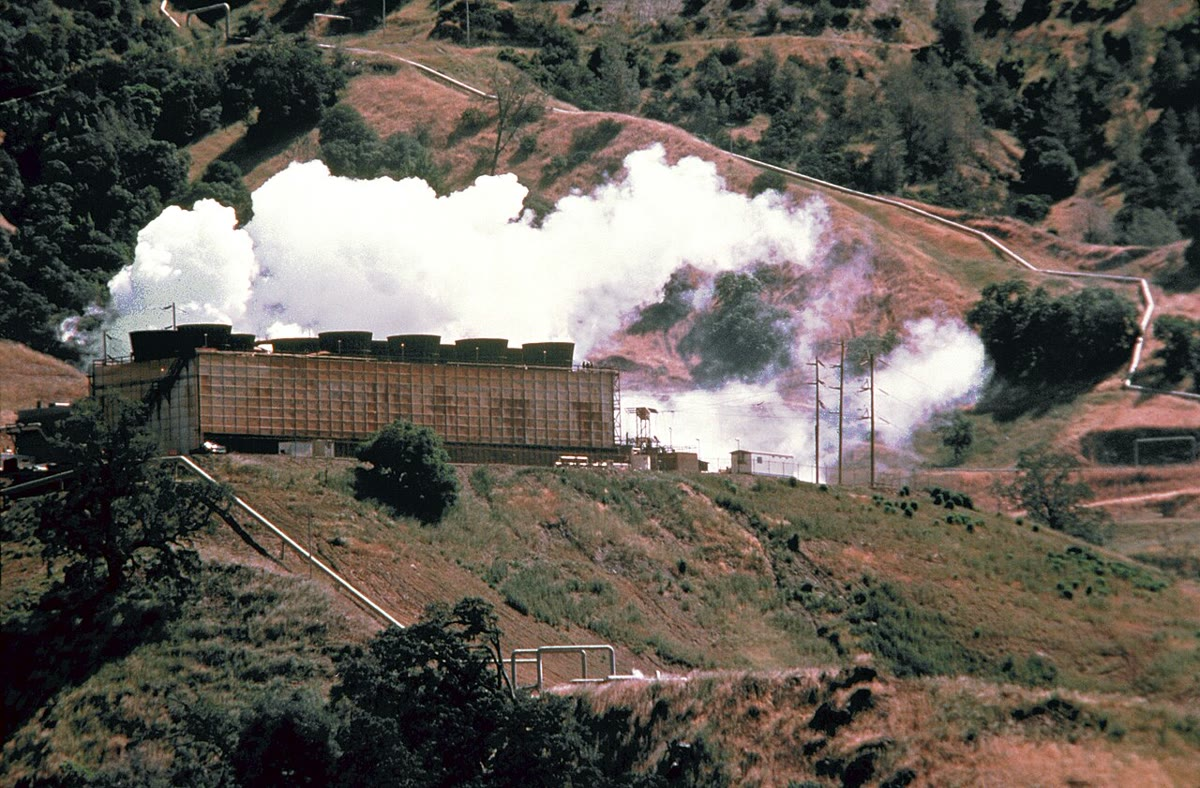
\includegraphics[width=\linewidth]{images/book4/b2-30-geyserville.jpg}
\end{minipage}
\par\smallskip{\small 左：高焓\omterm{def:b2:energy-geology:geothermal}{地热系统}（示意图，未按比例）：在边缘补给的
水（蓝色）经侵入体加热，穿过裂缝性储层
（红色）上升至温泉；水井从储层取水。右：盖泽维尔附近的地热发电厂，
位于加利福尼亚州，摄于 1982 年，山坡上有蒸汽管道。照片：U.S. Department of Defense
（公有领域）。}
\end{omfigure}
% ledger: photo:b2-30-geyserville, usgs08g:egs

\begin{definition}[诱发地震活动]\label{def:b2:energy-geology:induced}
\emph{诱发地震活动}\index{诱发地震活动}是由人为活动引起的地震活动，
这些活动改变地壳中的应力或孔隙流体压力，最常见的是
向地下注入流体。
\end{definition}

其机制为考虑孔隙流体压力的库仑判据：断层在切应力
达到 $\mu(\sigma_n - p)$ 时发生滑动，因此提高 $p$ 会使已受应力的断层趋于破裂，
构造荷载无任何变化。20 世纪 60 年代，在丹佛附近
落基山兵工厂之下、深度为 3.7 至
\qty{7.0}{km} 的破裂前寒武纪基底中注入废液，引发了地震；地震局限于储层中
压力升高超过 \qty{32}{bar}（\qty{3.2}{MPa}）的部分。俄克拉何马州地震活动的急剧增加
被\omterm{def:b2:anthropogenic-climate-change:da}{归因}于废水处置：四口大流量
注水井可能占美国中部地震活动的五分之一，并引发
超过 \qty{30}{km} 远处的地震。刺激\omterm{def:b2:energy-geology:geothermal}{增强型地热系统}储层时，
会以同样方式、有意地提高孔隙压力。
% ledger: hb81:denver, keranen:oklahoma, usgs08g:egs

\section{铀}\label{sec:b2:energy-geology:uranium}

两类\omterm{def:b2:ore-deposits:types}{矿床类型}说明铀如何富集：一类位于古老的不整合面，
另一类位于砂岩中。

\begin{definition}[不整合面型和卷状铀矿床]\label{def:b2:energy-geology:uranium}
\emph{不整合面型铀矿床}\index{不整合面型铀矿床}是一个矿体，
由沥青铀矿和晶质铀矿充填于变质含碳泥质岩中的裂隙与角砾岩，并
赋存于其上、下或横跨不整合面的石英砂岩中，该不整合面位于早、中
元古代岩石之间，位于\omterm{def:b2:basins-compared:types}{克拉通内盆地}中。一种\emph{卷状铀矿床}\index{卷状铀矿床}
是一种新月形的铀矿物矿体，横切
长石质或凝灰质砂岩的层理，位于氧化带与还原带的交界处，
铀在局部还原环境中沉积，并与黄铁矿共生。
\end{definition}

不整合面型\omterm{def:b2:ore-deposits:deposit}{矿床}的主岩为 1800 至 \qty{1200}{\Ma} 的岩石，即不整合面下方的变质
泥质岩和其上未变质的砂岩；其主岩已绿泥石化，伴生许多\omterm{def:b2:ore-deposits:deposit}{矿床}的石墨片岩
是强导电体，是电磁勘测的目标。典型例子有萨斯喀彻温省的
基湖、克拉夫湖和兔湖，以及澳大利亚北部的贾比卢卡和兰杰，
皆为此类实例。卷状\omterm{def:b2:ore-deposits:deposit}{矿床}形成较晚，多为第三纪：在由长英质火山灰或
花岗岩供给物质的砂岩中，氧化态铁矿物位于前缘的上倾方向，还原态者位于下倾方向，如
怀俄明州与得克萨斯墨西哥湾沿岸的盆地所示。
% ledger: b1693:unconformity, b1693:sandstone

\begin{proposition}[过去的铀-235]\label{prop:b2:energy-geology:u235}
设 $r_0$ 为今日的原子比 $^{235}$U/$^{238}$U，$\lambda_5$、$\lambda_8$ 为两种同位素的
衰变常数。$t$ 以前的比值为
\begin{equation}
r(t) = r_0\,e^{(\lambda_5 - \lambda_8)\,t} ,
\label{eq:b2:energy-geology:u235}
\end{equation}
$^{235}$U 占铀原子的份额为 $r/(1 + r)$，略去
$^{234}$U 的痕量。
\end{proposition}

\begin{proof}
每种同位素均按指数规律衰变：$N_5(\text{现在}) = N_5(t)\,e^{-\lambda_5 t}$ 和 $N_8(\text{现在})
= N_8(t)\,e^{-\lambda_8 t}$。两式相除，$r_0 = r(t)\,e^{-(\lambda_5 - \lambda_8)t}$。
\end{proof}

取 $\lambda_5 = \qty{9.8485e-10}{\text{年}^{-1}}$，$\lambda_8 = \qty{1.55125e-10}{\text{年}^{-1}}$，今日的
丰度分别为 \qty{0.7204}{\percent} 和 \qty{99.2742}{\percent}，$r_0 = 0.0072567$；\qty{2.0}{\Ga}
以前 $r = 0.0381$，天然铀中 $^{235}$U 占 \qty{3.67}{\percent}，是今日的
份额的五倍。
% ledger: amherst:constants, iaea:isotopes
% values: r 0.038144, 3.6743 % (calc/ch30.py)

\begin{history}[二十亿年前的天然反应堆]
1972 年，法国科学家在测量铀矿石时，发现了微小但显著的
$^{235}$U 亏损，他们将其追溯到加蓬的奥克洛矿。那里的岩块，
含铀高达 \qty{65}{\percent}，其中 $^{235}$U 的份额低至正常值的一半，钕
的原始同位素 $^{142}$Nd 亏损，而富集的是裂变
产生的 143 至 150 号同位素：约二十亿年前，矿石中曾发生链式反应，压强约为 \qty{300}{bar}，
温度为 400 至 \qty{500}{\celsius}。已知的此类天然反应堆共十六座，位于奥克洛及邻近的
邦贡贝（Bangombé），是世界上仅有的两处发现地；有机物曾帮助
铀富集，此后铀氧化物一直将大部分锕系元素和
不挥发的裂变产物留存于原处。
\end{history}
% ledger: oklo:curtis, oklo:cowan, oklo:gl96, oklo:nagy

\section{地质封存二氧化碳}\label{sec:b2:energy-geology:ccs}

\begin{definition}[地质 \ce{CO2} 封存、圈闭机制、封存效率系数]\label{def:b2:energy-geology:ccs}
\emph{地质 \ce{CO2} 封存}\index{地质 CO$_2$ 封存}是指将二氧化碳注入
深埋地下的多孔岩层、已枯竭的油气藏、深部咸水层
或煤层中，以便长期滞留。\emph{\ce{CO2} 圈闭
机制}\index{CO$_2$ 圈闭机制}包括：盖层之下的构造（及地层）圈闭；
剩余圈闭，即以毛细力保持在孔隙中的不可动相；
溶解圈闭，即溶解于地层水中；矿物圈闭，即与矿物反应生成碳酸盐；
以及在煤和页岩中，吸附于有机质上。地层的\emph{封存效率系数}\index{封存效率系数}
$E$ 为其孔隙体积中预计可被注入的
\ce{CO2} 所能充满的比例。
\end{definition}
% ledger: srccs:retention, netl08:saline

二氧化碳在地表为气体，但其临界点位于 \qty{31.0}{\celsius} 和
\qty{7.38}{MPa}。沿地温梯度 \qty{25}{\celsius\per\km}、自 \qty{15}{\celsius} 起算，在静水压力下，
温度在 \qty{641}{m} 深处越过临界值，压强则在
\qty{742}{m} 深处越过；纯 \ce{CO2} 的密度在 \qty{700}{m} 处由 \qty{234}{kg.m^{-3}} 跃升至
\qty{583}{kg.m^{-3}}（\qty{900}{m} 处），此后
在 \qty{1.5}{km} 以下趋于平稳，约为 670 至 \qty{700}{kg.m^{-3}}。一吨二氧化碳在地表占 \qty{534}{m^3}，在 \qty{1000}{m} 处占 \qty{1.6}{m^3}，
体积缩小了 330 倍，这正是封存评估只考虑深于
\qty{800}{m} 的地层的原因。
% ledger: nist:co2-critical, data:b4-co2-density, srccs:density, netl08:saline
% values: z_tc 641.2 m, z_pc 742.2 m; volume ratio 331.9 (figdata co2_density.py numbers)

\begin{omfigure}
\centering
\begin{minipage}[b]{0.49\linewidth}\centering
\begin{tikzpicture}
\begin{axis}[omrecord, width=0.95\linewidth, height=5.2cm, xmin=0, xmax=750, ymin=0, ymax=3,
  y dir=reverse, xlabel={\ce{CO2} 密度（\unit{kg.m^{-3}}）}, ylabel={深度（km）},
  tick label style={font=\scriptsize}, label style={font=\small}]
% computed in figdata/bachelor-2/co2_density.py part profile; ledger: data:b4-co2-density
\addplot[black!45, densely dashed] coordinates {(0,0.742) (750,0.742)};
\node[font=\tiny, text=black!60, anchor=south east] at (axis cs:745,0.73) {临界压强};
\addplot[omDef, line width=1.1pt, mark=*, mark size=0.9pt] table[x=rho, y expr=\thisrow{depth_m}/1000] {figdata/out/bachelor-2-co2_density-profile.dat};
\end{axis}
\end{tikzpicture}
\end{minipage}\hfill
\begin{minipage}[b]{0.49\linewidth}\centering
\begin{tikzpicture}
\begin{axis}[width=0.95\linewidth, height=5.2cm, xmin=0, xmax=4, ymin=0, ymax=100,
  axis x line=bottom, axis y line=left, axis line style={-}, axis on top,
  xlabel={注入后时间（年）}, ylabel={已封存 \ce{CO2} 的份额},
  xtick={0,1,2,3,4}, xticklabels={1,10,100,1000,$10^4$}, ytick=\empty,
  tick label style={font=\scriptsize}, label style={font=\small}]
% schematic, after IPCC SRCCS (2005) Figure 5.9; ledger: srccs:trapping
% bands from the bottom: mineral, solubility, residual, structural (cumulative tops 0/0/1/5/15,
% 2/8/21/40/60, 10/30/56/80/90, 100)
\fill[omLithLime!60!black] (axis cs:0,0) -- (axis cs:1,0) -- (axis cs:2,1) -- (axis cs:3,5) -- (axis cs:4,15) -- (axis cs:4,0) -- cycle;
\fill[omDef!40] (axis cs:0,0) -- (axis cs:1,0) -- (axis cs:2,1) -- (axis cs:3,5) -- (axis cs:4,15) -- (axis cs:4,60) -- (axis cs:3,40) -- (axis cs:2,21) -- (axis cs:1,8) -- (axis cs:0,2) -- cycle;
\fill[omProp!40] (axis cs:0,2) -- (axis cs:1,8) -- (axis cs:2,21) -- (axis cs:3,40) -- (axis cs:4,60) -- (axis cs:4,90) -- (axis cs:3,80) -- (axis cs:2,56) -- (axis cs:1,30) -- (axis cs:0,10) -- cycle;
\fill[black!15] (axis cs:0,10) -- (axis cs:1,30) -- (axis cs:2,56) -- (axis cs:3,80) -- (axis cs:4,90) -- (axis cs:4,100) -- (axis cs:0,100) -- cycle;
\node[font=\scriptsize] at (axis cs:1.1,72) {构造圈闭};
\node[font=\scriptsize] at (axis cs:2.1,38) {剩余圈闭};
\node[font=\scriptsize] at (axis cs:3.1,22) {溶解圈闭};
\node[font=\scriptsize, text=white, anchor=south east] at (axis cs:3.98,0.5) {矿物圈闭};
\end{axis}
\end{tikzpicture}
\end{minipage}
\par\smallskip{\small 左图：纯 \ce{CO2} 密度随深度的变化，沿地温梯度
\qty{25}{\celsius\per\km}、自 \qty{15}{\celsius} 起算，静水压力下。数据来自 NIST Chemistry
WebBook（Span--Wagner 状态方程），计算条件参照 IPCC 特别报告
Carbon Dioxide Capture and Storage（2005）。右图：各圈闭机制随时间如何分担已封存的 \ce{CO2}
（示意图，取自同一报告）：盖层圈闭逐步让位于剩余圈闭、溶解圈闭和矿物圈闭，
这些形式的流动性较弱。}
\end{omfigure}

\begin{proposition}[地层的封存容量]\label{prop:b2:energy-geology:capacity}
设地层面积为 $A$、厚度为 $h$、孔隙度为 $\phi$，其中 \ce{CO2} 的密度为 $\rho$，
\omterm{def:b2:energy-geology:ccs}{封存效率系数}为 $E$，则可封存的质量为
\begin{equation}
M = A\,h\,\phi\,\rho\,E .
\label{eq:b2:energy-geology:capacity}
\end{equation}
对于已枯竭的油田，若其采出的地面体积为 $N_p$，按等体积替换所采出的原油，
则 $M = \rho\,N_p\,B_o$。
\end{proposition}

\begin{proof}
孔隙体积为 $Ah\phi$，其中 \ce{CO2} 所占比例为 $E$，密度为 $\rho$。在
油田中，已采出的原油在储层中占 $N_pB_o$，即为 \ce{CO2} 所取代的体积。
\end{proof}

对于深部咸水层，模拟给出 $E$ 介于孔隙体积的 1 至 \qty{4}{\percent} 之间，
在 15\% 至 85\% 的置信区间内，中位数约为 \qty{2}{\percent}：大部分孔隙
空间永远无法被触及，或仍保留其中的水。一个面积为 \qty{1000}{km^2}、厚 \qty{50}{m} 的
地层，孔隙度为 0.20、位于 \qty{2000}{m} 深处（$\rho = \qty{686}{kg.m^{-3}}$），可封存 \qty{137}{Mt} 二氧化碳（取 $E =
\qty{2}{\percent}$）。
% ledger: netl08:saline, data:b4-co2-density
% values: 1e9*50*0.2*686*0.02 = 1.372e11 kg (calc/ch30.py)

注入之后，\ce{CO2} 在盖层之下上升并扩散。在运移羽流的后方，毛细力
保持的剩余饱和度可达孔隙空间的 15 至 \qty{25}{\percent}；
溶解作用使每立方米地层水可容纳 20 至 \qty{60}{kg} 的 \ce{CO2}，而在
流动缓慢的地层中，多达 \qty{30}{\percent} 的注入 \ce{CO2} 会在数十
年内溶解。溶解圈闭主要在数十至数百年内起作用，离子态则在数百至
数千年内起主导作用，矿物圈闭则在数千至数百万年内占主导：与碳酸盐矿物的反应只需数天，
与硅酸盐矿物的反应则需数百至数千年。封存随时间推移而更加可靠，在
选址与管理均妥善的场地，\qty{99}{\percent} 或更多的 \ce{CO2} 在
1000 年内得以留存被认为很可能。
% ledger: srccs:trapping, srccs:retention

\begin{dated}{2005}
在挪威以西约 \qty{250}{km} 的北海，斯莱普内尔气田天然气中分离出的 \ce{CO2}，
约占该气田天然气的 \qty{9}{\percent}，自 1996 年 10 月起注入
海底以下 800 至 \qty{1000}{m} 处的乌特西拉组，一种未固结的含盐砂岩，
注入速率约每年 \qty{1}{Mt}。截至 2005 年初，在计划于项目全周期内封存的 \qty{20}{Mt} 中，已封存超过 \qty{7}{Mt}。
多次地震勘测对羽流成像，当时其平面范围约为
\qty{5}{km^2}，勘测显示其上方的盖层将其封闭。
\end{dated}
% ledger: srccs:sleipner

\begin{inthefield}[钻井过程中读取井孔资料]
\centering
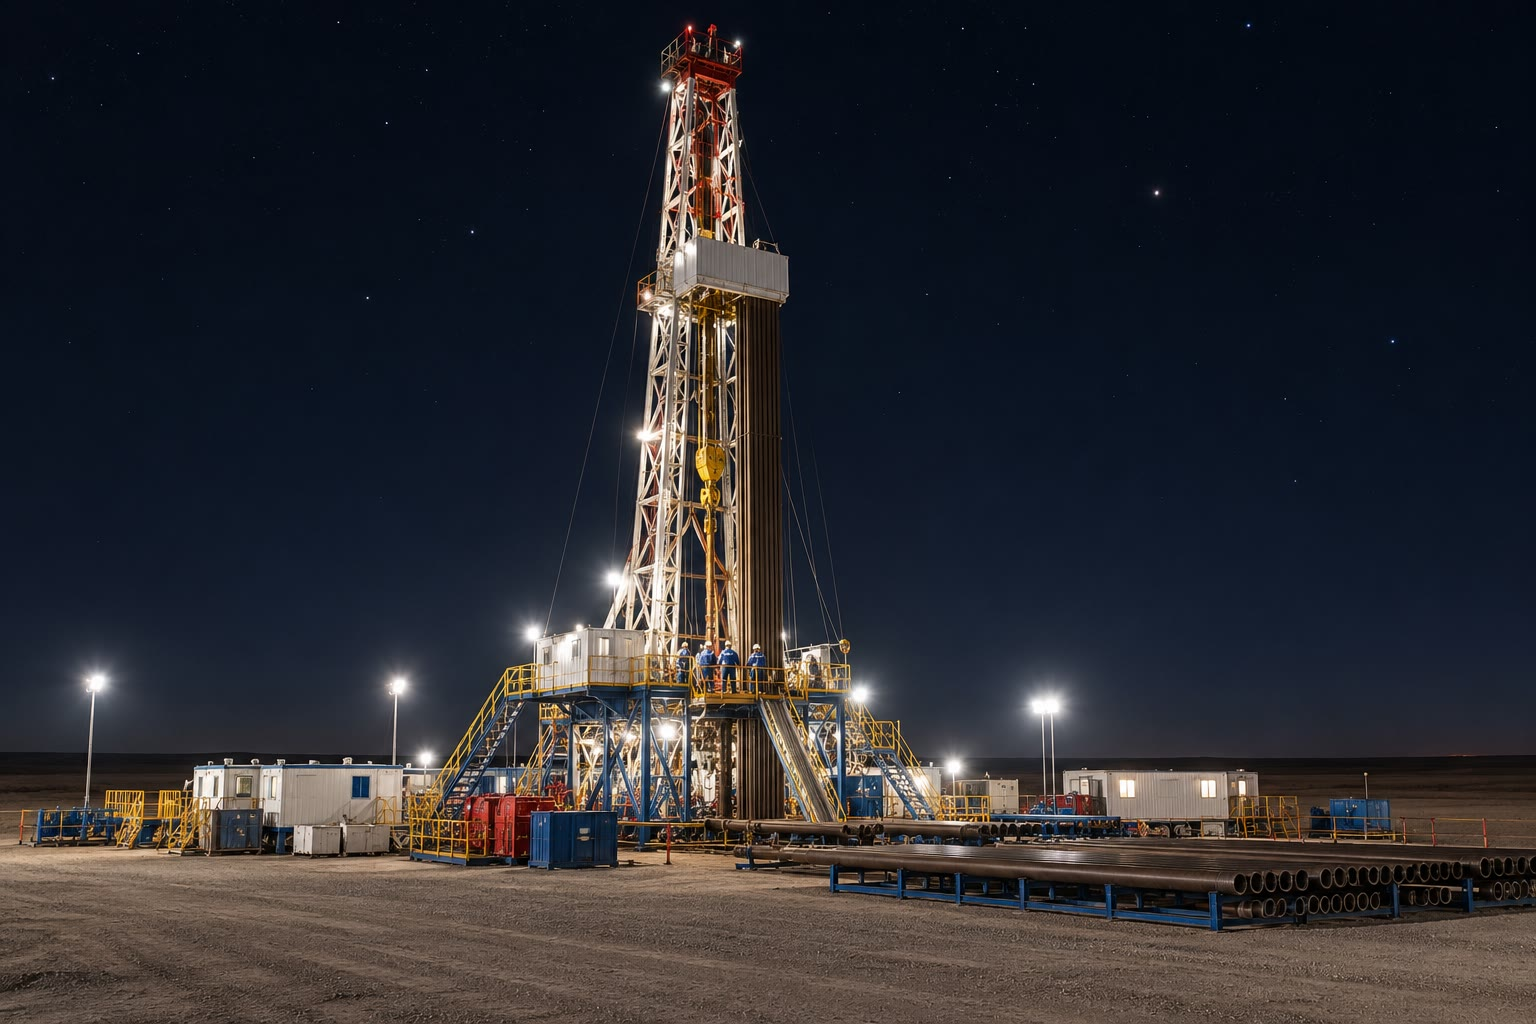
\includegraphics[width=0.56\linewidth]{images/book4/ai/b2-rig-night.jpg}
\par\smallskip{\small 夜间的陆地钻机（AI 生成插图）。}
\par\medskip\raggedright
当一段井孔完成后，地球物理学家用电缆将仪器放入井中，
沿深度记录井周岩石的性质：一是天然放射性，砂岩中较低，
页岩中较高；另一是体积密度，据此可算出孔隙度，
其公式为（颗粒密度 $-$ 体积密度）/（颗粒密度 $-$ 流体密度），其中石英颗粒取 \qty{2.65}{g/cm^3}，
水取约 \qty{1}{g/cm^3}。综合这些井孔测井，
可得出净储层厚度和孔隙度，二者即为本章体积公式所用的参数。
\end{inthefield}
% ledger: keys:gamma, keys:density-porosity

\section*{练习}\label{sec:b2:energy-geology:exercises}

除另有说明外，练习所用数据如下：$R = \qty{8.314}{J.mol^{-1}.K^{-1}}$；一百万
年为 \qty{3.156e13}{s}；格林河干酪根 $A = \qty{9.21e13}{s^{-1}}$，$E/R = \qty{26800}{K}$；
原子质量 C 12.011、H 1.008、O 15.999；图中剖面上 \ce{CO2} 的密度：
地表为 \qty{1.872}{kg.m^{-3}}，在 \qty{900}{m} 处为 583，在 \qty{1000}{m} 处为 621，在
\qty{2000}{m} 处为 686。结果保留三位有效数字。
% ledger: codata:R, fp14:gr-daem, data:b4-co2-density

\begin{exercise}[$\star$]\label{exo:b2:energy-geology:1}
(a) 四种未成熟干酪根的原子 H/C 分别为 1.58、0.95、1.24 和 1.12。判定每种干酪根的类型，并说明
哪一种主要生成天然气。(b) 核对化学式的 H/C 与 O/C 比值，
C$_{100}$H$_{150}$N$_3$O$_8$S。(c) 由质量组成 C \qty{77.4}{\percent}、H
\qty{9.8}{\percent}、O \qty{8.2}{\percent} 求出这些比值。
\end{exercise}

\begin{exercise}[$\star$]\label{exo:b2:energy-geology:2}
(a) 五个 II 型烃源岩样品的 $R_o$ 分别为 0.45、0.68、1.1、1.6 和 \qty{2.5}{\percent}。
说明每个样品在生油、生气方面所处的状态。(b) III 型干酪根在 $R_o =
\qty{0.68}{\percent}$ 时是否正在生成甲烷？(c) Easy\%Ro 的哪一转化率 $F$ 对应于
$R_o = 0.6$ 和 \qty{1.3}{\percent}？
\end{exercise}

\begin{exercise}[$\star$]\label{exo:b2:energy-geology:3}
某圈闭面积为 \qty{6}{km^2}，储层净厚度为 \qty{25}{m}，孔隙度为 0.18，水饱和度为
0.30，体积系数 $B_o = 1.25$。(a) 求储层中油的体积及 STOIIP。(b) 求
\omterm{def:b2:energy-geology:volumetrics}{采收率}分别为 0.30 和 0.40 时的采出油量。
\end{exercise}

\begin{exercise}[$\star$]\label{exo:b2:energy-geology:4}
某砂岩含水层厚 \qty{200}{m}，面积为 \qty{10}{km^2}，温度为 \qty{75}{\celsius}。(a) 求其高于
\qty{15}{\celsius} 的\omterm{def:b2:energy-geology:geothermal}{地热储量}，取 $C = \qty{2.5}{MJ.m^{-3}.K^{-1}}$。(b) 据此按焓值划分，它属于
哪一类资源？(c) 求 30 年内的平均热功率，取 $R_g = 0.25$。
\end{exercise}

\begin{exercise}[$\star\star$]\label{exo:b2:energy-geology:5}
(a) 求使阿伦尼乌斯速率在 100 至
\qty{110}{\celsius} 之间增为两倍的活化能。(b) 在同一区间内，格林河反应速率增大为原来的多少倍，
(c) 两种规则中，哪一种更重视岩石在低温下停留的时间，
以及这对 I 型烃源岩计算的 TTI 有何意味？
\end{exercise}

\begin{exercise}[$\star\star$]\label{exo:b2:energy-geology:6}
(a) 由 \eqref{eq:b2:energy-geology:maturation} 证明，半转化温度满足
$T = (E/R)\big/\ln\bigl[A T^2/(\beta\,(E/R)\ln 2)\bigr]$，并用迭代法求解格林河干酪根在
以 \qty{1}{\celsius\per\Ma} 及每分钟 \qty{10}{K} 的速率加热时的温度。(b) 比较这一差值与
在较低温度下取值的估计式 $(RT^2/E)\ln(\beta_2/\beta_1)$，并
解释两者差异的原因。
\end{exercise}

\begin{exercise}[$\star\star$]\label{exo:b2:energy-geology:7}
利用 \eqref{eq:b2:energy-geology:u235} 及正文数据：(a) 求 $^{235}$U 在
天然铀中的占比，分别为距今 \qty{2.0}{\Ga} 与 \qty{1.8}{\Ga} 时的值；(b) 其占比为 \qty{3.00}{\percent} 是在何时？
(c) 奥克洛矿石中 $^{235}$U 的占比仅为今日正常值的一半。忽略 $^{238}$U
的消耗，则反应时存在的 $^{235}$U 中被裂变的比例为多少，并
为何此后的衰变不会改变结果？
\end{exercise}

\begin{exercise}[$\star\star$]\label{exo:b2:energy-geology:8}
(a) 求 \qty{1}{Mt} 的 \ce{CO2} 在地表、\qty{1000}{m} 处及
\qty{2000}{m} 处的体积。(b) 截至 2005 年，斯莱普内尔已注入超过 \qty{7}{Mt}，位于约
\qty{900}{m} 处、面积为 \qty{5}{km^2} 的羽流中。取孔隙度为 0.35，\ce{CO2} 的
饱和度为 0.30，求其所占岩石的体积及平均厚度。
\end{exercise}

\begin{exercise}[$\star\star$]\label{exo:b2:energy-geology:9}
一高焓储层尺寸为 $3 \times 2 \times \qty{1.5}{km}$，温度为 \qty{250}{\celsius}，
热容 $C = \qty{2.6}{MJ.m^{-3}.K^{-1}}$。(a) 求其高于 \qty{15}{\celsius} 的\omterm{def:b2:energy-geology:geothermal}{地热储量}。(b) 求
30 年内的平均热功率（$R_g = 0.1$ 和 $0.25$）。(c) 其地热田面积为 \qty{6}{km^2}；
若每平方千米发电量为 10 至 \qty{20}{MW}，则在
$R_g = 0.1$ 时的热功率中有多大比例转化为电力？
\end{exercise}

\begin{exercise}[$\star\star\star$]\label{exo:b2:energy-geology:10}
某断层位于约 \qty{4}{km} 深处，正应力为 \qty{80}{MPa}，切应力为
\qty{22}{MPa}；其摩擦系数为 0.6，孔隙压力为静水压力，
即 \qty{39}{MPa}。(a) 该断层是否稳定？求使其失稳的孔隙压力升高量，分别以
兆帕和巴表示，并与丹佛阈值比较。(b) 若切应力为
\qty{24}{MPa}，求同样的量。(c) 解释为何诱发地震可发生在离注入井数千米之外，
以及在注入开始数年之后。
\end{exercise}

\begin{exercise}[$\star\star\star$]\label{exo:b2:energy-geology:11}
(a) 由 \eqref{eq:b2:energy-geology:maturation} 中的近似式，证明在恒定升温速率下，
转化率由 \qty{10}{\percent} 升至 \qty{90}{\percent} 所跨越的
温度区间 $\Delta T \approx \bigl[\ln\ln 10 - \ln\ln(10/9)\bigr]\,RT^2/E$。(b) 计算其值，
取格林河干酪根在 \qty{1}{\celsius\per\Ma} 下的情形。(c) 与图中实线比较，
并解释两者差异。
\end{exercise}

\begin{exercise}[$\star\star\star$]\label{exo:b2:energy-geology:12}
Sleipner 拟封存 \qty{20}{Mt} 的 \ce{CO2}。(a) 求溶解全部该气体所需的
地层水体积，分别取 20 与 \qty{60}{kg.m^{-3}}；(b) 求其以游离相存在于
\qty{1000}{m} 处时的体积。(c) 取 $E = \qty{2}{\percent}$，求所需地层的孔隙体积，并
求厚 \qty{50}{m}、孔隙度为 0.30 的地层面积。
\end{exercise}
% ledger: srccs:trapping, srccs:sleipner, hb81:denver

\begin{problem}[{周末问题——一个盆地，两种用途}]\label{pb:b2:energy-geology:1}
在一个虚构的盆地中，I 型烃源岩于 \qty{120}{\Ma} 在地表沉积。
随后沉积物以每百万年 \qty{60}{m} 的速率堆积，直至 \qty{70}{\Ma}，此后以
每百万年 \qty{30}{m} 的速率堆积至今。地表温度为 \qty{15}{\celsius}，地温线
保持恒定，为 \qty{25}{\celsius\per\km}。干酪根采用正文中的格林河动力学（单一活化能）。
其生油区，即烃源岩中已成熟的部分，面积为 \qty{400}{km^2}，厚 \qty{50}{m}，且
密度为 \qty{2400}{kg.m^{-3}}，完全转化时每吨岩石可产油 \qty{30}{kg}，
原油的地面密度为 \qty{850}{kg.m^{-3}}。原油充满一个
\qty{12}{km^2} 的圈闭，其储层中心深度为 \qty{2000}{m}，净厚度为 \qty{40}{m}，
孔隙度为 0.22，含水饱和度为 0.25，$B_o = 1.30$。沿用练习中的数据，
结果取三位有效数字。

\noindent\textbf{第一部分——埋藏与\omterm{def:b2:energy-geology:maturity}{时间–温度指数}。}
\begin{enumerate}
  \item 求烃源岩在 \qty{70}{\Ma} 时及今天的深度和温度。
  \item 求各阶段的升温速率。
  \item 求烃源岩在每个 \qty{10}{\celsius} 的温度区间内所经历的时间，
        温度自 \qty{15}{\celsius} 升至现今温度。
  \item 按正文方法计算其现今的 TTI。
  \item 何时、在何温度及何深度处，其 TTI 达到 15？
  \item 对 TTI 为 75 与 160 的情形，求同样的量。
  \item 由 TTI 判断，烃源岩是否仍在生油？
\end{enumerate}

\noindent\textbf{第二部分——动力学转化。}
\begin{enumerate}[resume]
  \item 求 \qty{90}{\celsius} 时的速率常数，并证明在 \qty{70}{\Ma} 之前，
        被转化的干酪根不足 \qty{0.2}{\percent}。
  \item 由 \eqref{eq:b2:energy-geology:maturation}，取第二阶段的升温速率，
        求现今的未转化分数与转化率。
  \item 求该升温速率下转化一半时的温度（练习~\ref{exo:b2:energy-geology:6}）。
  \item 何时达到该温度？
  \item 将其与由 TTI 给出的生油高峰时间相比较，并解释差异。
  \item 若为平均活化能较低的 II 型干酪根，其转化会更早还是更晚？
\end{enumerate}

\noindent\textbf{第三部分——生成、就地及可采的石油。}
\begin{enumerate}[resume]
  \item 取转化率为 0.92，求生油区生成的石油质量。
  \item 求其在地面条件下的体积。
  \item 求圈闭的 STOIIP（地面条件下的原始地质储量）。
  \item 圈闭所含油量占生成油量的比例是多少？对 (15) 取 \qty{1.56e9}{m^3}。
  \item 求\omterm{def:b2:energy-geology:volumetrics}{采收率}为 0.35 时的产油量。
  \item 为何\omterm{def:b2:energy-geology:volumetrics}{采收率}远小于 1？注入 \ce{CO2} 会带来怎样的改变？
\end{enumerate}

\noindent\textbf{第四部分——枯竭油田作为 \ce{CO2} 储库。}
\begin{enumerate}[resume]
  \item 求储层的温度和静水压力。注入的 \ce{CO2} 在该处
        是否处于超临界状态？请由图中读出其密度。
  \item 取 $N_p = \qty{2.13e7}{m^3}$，求因生产而释放出的储层体积。
  \item 将其表示为圈闭孔隙体积的储存效率系数，并与
        咸水层相比较。
  \item 油田下方的一层咸水层面积为 \qty{600}{km^2}，厚 \qty{80}{m}，
        孔隙度为 0.20，其中 \ce{CO2} 密度为 \qty{691}{kg.m^{-3}}。求其在 $E =
        \qty{2}{\percent}$ 时的容量。
  \item 以 Sleipner 的注入速率计，注满它需要多少年？
  \item 取 $\rho = \qty{686}{kg.m^{-3}}$，并将释放出的体积取整为 \qty{2.77e7}{m^3}，求
        枯竭储层的 \ce{CO2} 储存容量，单位为百万吨。
\end{enumerate}
\end{problem}
% ledger: fp14:gr-daem, waples80:tti, hamm14:tti-table, netl08:oilgas, netl08:saline, data:b4-co2-density, nist:co2-critical, srccs:sleipner
